\chapter{Anwendung zur TLS-Simulation}
\label{cha_implementation}

Dieses Kapitel widmet sich der im Rahmen dieser Arbeit entwickelten Anwendung. 
Die Anwendung ist speziell für den Einsatz in der Hochschullehre gedacht. Sie soll dazu dienen, Protokolle und ihre internen Abläufe darzustellen, und soll durch zusätzliche Interaktivität exploratives Lernen ermöglichen. Eine Vorgabe war es, die Möglichkeit zur Erweiterung der Anwendung um weitere Protokolle vorzusehen. 

Im ersten Abschnitt werden allgemeine Entscheidungen erläutert, die getroffen wurden, um diese Vorgabe zu berücksichtigen.Außerdem werden Überlegungen für die Erweiterung der Anwendung um das TLS-Protokoll dargelegt.\\
Anschließend wird die Implementation beschrieben, wobei zuerst auf die Umsetzung der allgemeinen Anwendung eingegangen wird und dann auf die konkrete Umsetzung des TLS-Protokolls.

In Anhang \ref{cha_tutorial_plugin} werden anhand eines Beispiels einige Hinweise gegeben, was bei der Erweiterung der Anwendung um weitere Protokolle zu beachten ist.

\section{Analyse und Entwurf}

\subsection{Abstrakter Rahmen für die Anwendung}

Um die Vorgabe der Erweiterbarkeit zu ermöglichen, wurden zu Beginn der Entwicklungsarbeit die Gemeinsamkeiten von Protokollen herausgearbeitet, um diese abstrakt umsetzen zu können. So müssen anschließend lediglich protokollspezifische Eigenschaften in Erweiterungen implementiert werden.

Die Anwendung beschränkt sich auf Protokolle mit zwei Parteien. Zwischen diesen Parteien werden Nachrichten eines festen Formats (sogenannte Protokolldateneinheiten) über einen Kanal ausgetauscht. Die Abfolge verschiedener Nachrichtentypen und die bei ihrem Empfang stattfindenden Verarbeitungsschritte sind durch das Protokoll festgelegt. Zusätzlich besitzen die Parteien einen internen Zustand\footnote{
	Um Verwechslungen mit den im nächsten Absatz eingeführten Automatenzuständen zu vermeiden, wird der Zustand einer Partei im Folgenden immer als interner Zustand bezeichnet.
}, der beispielsweise als Resultat empfangener Nachrichten verändert werden kann. 

Aus diesen Voraussetzungen wurde ein abstrakter Rahmen entwickelt, der für konkrete Protokolle erweitert werden muss.\\
Für ein Protokoll sollte ein Nachrichtentyp bestehen, der von den Parteien gesendet und empfangen werden kann. Dazu muss ein Kanal zwischen den Parteien vorhanden sein, über den das Senden geschehen kann.

Um die Parteien, ihre internen Zustände und die Verarbeitungsschritte bei Nachrichtenempfang strukturiert entwickeln zu können, werden die Parteien als endliche Automaten betrachtet. Es können verschiedene Zustände implementiert werden, um strukturiert unterschiedliches Verhalten bei dem Erhalt von Nachrichten zu erreichen. Der Automat besitzt jeweils immer genau einen aktuellen Zustand, an den eingehende Nachrichten weitergeleitet werden. Abhängig vom gewünschten Verhalten können aus dem aktuellen Zustand heraus der aktuelle Zustand neu gesetzt und Nachrichten gesendet werden. Der Automat kann seinen Zuständen zusätzlich Zugriff auf den internen Zustand der Partei bereitstellen.

\begin{figure}
	\centering
	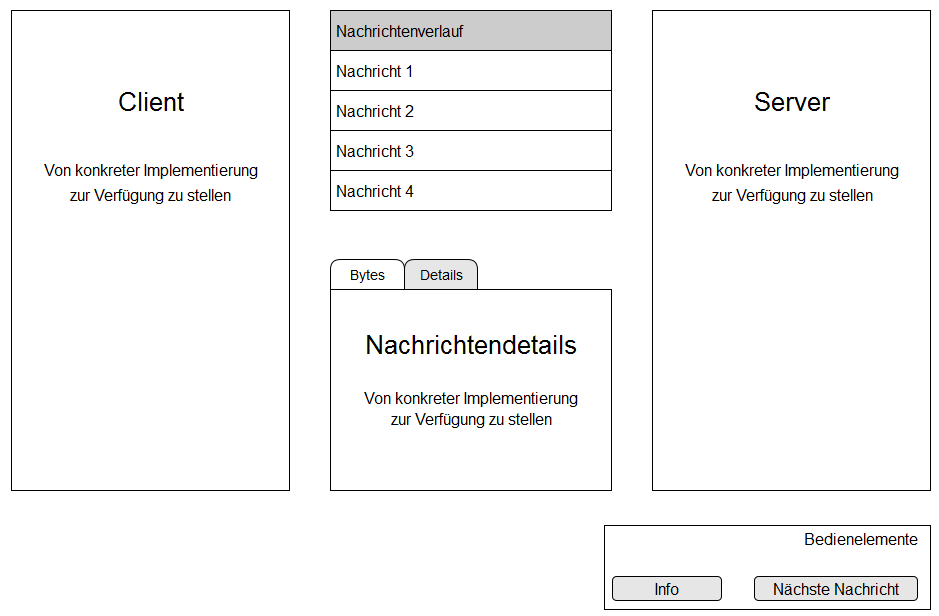
\includegraphics[width=15cm]{Diagrams/SketchUI.png} %
	\caption{Prototyp für die Benutzeroberfläche}
	\label{fig_ui_sketch}
\end{figure}

Anschließend wurde prototypisch eine Benutzeroberfläche entwickelt, die auf Basis dieser Überlegungen auch einen visuellen Rahmen bereitstellt, der für konkrete Protokolle gefüllt werden kann. Ein Prototyp ist in Abbildung \ref{fig_ui_sketch} zu sehen.\\
Es muss ermöglicht werden, den internen Zustand der beiden Parteien darzustellen, der jedoch vom betrachteten Protokoll abhängig ist. Ebenso soll zu jeder protokollabhängigen Nachricht, neben ihrer reinen Repräsentation als Bytefolge, auch die Möglichkeit angeboten werden, ihre Bedeutung darzustellen. Zusätzlich soll es möglich sein, dem Verlauf des Protokoll schrittweise zu folgen, um ablaufende Prozesse und Veränderungen an den internen Zuständen zu erkennen. Für das Verständnis des Protokollverhaltens bei (absichtlich oder unabsichtlich) veränderten Nachrichten ist auch eine Möglichkeit zum Bearbeiten von Nachrichten sinnvoll.\\
Mit diesen Möglichkeiten werden die Forderungen an exploratives Lernen und an Simulationen (siehe Abschnitt \ref{sec_exploration}), insbesondere der Perspektivenwechsel, die Anzeige nicht sichtbarer Prozesse und die Interaktivität, erfüllt.

\subsection{Erweiterung der Anwendung um TLS 1.2}
\label{sec_analysis_tls_plugin}

Für diese Arbeit wurde die TLS 1.2-Spezifikation als Erweiterung des abstrakten Rahmens umgesetzt. Hierdurch können die zum jetzigen Zeitpunkt aktuelle Version exploriert und insbesondere Abwehrmechanismen gegen Angriffe auf ältere Protokollversionen erkannt werden. Um diese Angriffe beobachten zu können, wäre auch die Umsetzung einer älteren Protokollversion wie SSL 2.0 nützlich. Durch die Erweiterbarkeit der Anwendung bietet sich hier die Möglichkeit für spätere Arbeiten.

Im ersten Schritt wurden für Client und Server auf Basis der TLS-Spezifikation Automatenmodelle entwickelt, die abhängig von empfangenen Nachrichten Zustandswechsel und gesendete Nachrichten abbilden. Die Modelle sind im Anhang \ref{cha_tls_state_machines} zu finden.\\
An den Zustandsübergängen sind jeweils die empfangenen Nachrichten in orange dargestellt, die zu diesem Übergang führen. Ist keine Nachricht angegeben, so findet direkt nach Eintritt in den Zustand der Zustandswechsel statt. Mit OnEnter gekennzeichnete Kästen an Zuständen zeigen in blau Nachrichten, die gesendet werden sollen, wenn ein Zustand aktueller Zustand wird. Kästen an Zustandsübergängen stehen für Aktionen, die von außen von dem Automaten verlangt werden (beispielsweise ein Verbindungsaufbauwunsch). In diese Kästen werden zu sendende Nachrichten ebenfalls in blau dargestellt. In eckigen Klammern werden Bedingungen für Zustandsübergänge und andere Aktionen angegeben. Der Startzustand wird durch die Unterstreichung des Namens gekennzeichnet.
 
Im zweiten Schritt wurde eine einfache Möglichkeit für die Darstellung der internen Zustände von Server und Client sowie für die Bedeutungsdarstellung von Nachrichten ausgearbeitet. Hierbei sollten insbesondere auch die Zustandsveränderungen kenntlich gemacht werden, um abgelaufene Vorgänge zu verdeutlichen. Die Wahl fiel auf eine baumartige Struktur aus Objekten, denen ein Titel und ein Wert sowie eine optionale Liste von Kindelementen zugewiesen werden kann. Veränderungen zwischen zwei Zuständen sollten durch Kennzeichnung der geänderten Objekte geschehen.

% Tls 1.2 nicht implementiert

Anschließend wurde die TLS-Spezifikation auf Funktionen untersucht, die aus Gründen der Komplexitätsreduktion nicht implementiert werden sollten, insbesondere wenn die Funktion wenig zum Verständnis der Zusammenhänge beigetragen hätte. Diese Funktionen und die Gründe, aus denen sie ausgelassen wurden, seien hier kurz dargestellt.

Auf TLS-Extensions wurde vollständig verzichtet, da sie für das grundsätzliche Verständnis von TLS nicht notwendig sind. Sie stellen eher technische Erweiterungen des Standards dar, um bestimmte Funktionen nachzurüsten oder um ein bestimmtes Verhalten zu erzwingen.

Auch die Möglichkeit, TLS-Plaintexte vor dem Verschlüsseln zu komprimieren, wurde nicht implementiert, da die Funktion wenig zum Verständnis beiträgt und zusätzlich aufgrund ihrer Angreifbarkeit in der nächsten Protokollversion wahrscheinlich nicht mehr enthalten sein wird (vgl. Abschnitt \ref{sec_attack_crime}).

TLS unterstützt optional zusätzliche Clientauthentifizierung. Diese wird allerdings in vielen Anwendungsfällen, wie bei dem verschlüsselten Abruf einer Internetseite über HTTPS, nicht genutzt und unterscheidet sich nicht übermäßig von der Serverauthentifizierung. Daher wurde auch auf diese Funktion in der Anwendung verzichtet.

Weiterhin wurden nur einige \ciphersuites{} implementiert. Hierbei wurden sowohl Block- und AEAD-Chiffren zur Ver- und Entschlüsselung als auch RSA und das Diffie-Hellman-Verfahren zum Schlüsselaustausch verwendet. Auf die Implementierung von \ciphersuites{}, die sich lediglich in Schlüssellängen von bereits implementierten \ciphersuites{} unterscheiden oder deren Chiffren bzw. Schlüsselaustauschalgorithmen bereits durch andere \ciphersuites{} abgedeckt waren, wurde bewusst verzichtet. Da von der Verwendung bereits abgeraten wird, wurde auch auf die Implementierung einer \ciphersuite{} mit der Stromchiffre RC4 verzichtet.

Auf die sichere Verwaltung von Schlüsseln im Dateisystem, sowie die Entfernung verwendeter Schlüssel aus dem Speicher, auf die in produktiv verwendeten Systemen geachtet werden muss, konnte hier aus naheliegenden Gründen verzichtet werden.

Zusätzlich wurden auch die Möglichkeit der Übertragung eigener Daten und zur Simulation von auf TLS aufsetzenden Protokollen wie HTTPS bei bestehender Verbindung nicht aufgenommen. Diese Funktion wäre jedoch beispielsweise für Betrachtungen zur Erkennung der Nachrichtenlänge oder zur Darstellung von Angriffen wie den in den Abschnitten \ref{sec_attack_beast} und \ref{sec_attack_crime} beschriebenen hilfreich.

Aus Zeitgründen wurde auch auf die Wiederaufnahme bestehender Sitzungen verzichtet (siehe Abschnitt \ref{sec_session_connection}). Der verkürzte Handshake hat eher praktische Bedeutung, da auf erneute Aushandlung kryptographischer Verfahren und damit mehrere Nachrichten während des Handshakes verzichtet werden kann und die Wiederaufnahme der Verbindung somit weniger Zeit in Anspruch nimmt. Eine spätere Erweiterung der Anwendung um diese Funktion wäre jedoch sinnvoll, um das Verständnis von TLS zu vertiefen.

Ein letzter Punkt, der in der Anwendung nicht implementiert wurde, ist die Zertifikatsvalidierung. Diese ist zwar entscheidend für den sicheren Aufbau einer Verbindung, hat aber eher indirekt mit der der Protokollspezifikation zu tun. Daher wurde zunächst auf diese Funktion verzichtet, die sich jedoch für spätere Arbeiten anbietet.

\section{Implementierung}

Die Wahl der Programmiersprache für die Anwendung fiel auf Java, da diese Sprache an der Universität Hamburg in der ersten Semestern zum Einsatz kommt und von den Studierenden zwingend gelernt werden muss. Auf diese Weise sollte die entwickelte Anwendung auch von anderen Studierenden erweitert oder zumindest problemlos verstanden werden können. Zur Erzeugung der Benutzeroberfläche wurde die in der Java-Runtime verfügbare Bibliothek Swing genutzt, da diese ebenfalls in einigen Veranstaltungen an der Universität Hamburg verwendet wird.

\subsection{Abstrakter Rahmen für die Anwendung}

% abstract model
Ein UML-Diagramm der entwickelten Klassen für den abstrakten Rahmen ist in Abbildung \ref{fig_uml_abstract_state_machine} aufgeführt. Diese Klassen sollen hier im Detail betrachtet.

Protokollnachrichten werden durch die abstrakte Klasse \sourceobject{ProtocolDataUnit} dargestellt. In Unterklassen muss die Byte-Repräsentation einer Nachricht sowie Titel und Untertitel für die Darstellung auf der Benutzeroberfläche implementiert werden.

Für den abstrakten Rahmen wurden die Parteien als endliche Automaten modelliert. Für diese Modellierung wurde das Entwurfsmuster Zustand eingesetzt. Details hierzu sind \cite{freeman04} zu entnehmen.\\
Die abstrakte Klasse \sourceobject{StateMachine} bildet das Grundgerüst für einen Automaten und die abstrakte Klasse \sourceobject{State} wurde zur Implementierung der jeweiligen Automatenzustände benutzt. In einem \sourceobject{StateMachine}-Objekt können der aktuelle Zustand gesetzt und abgefragt sowie Nachrichten gesendet werden. Die möglichen Zustände müssen dem Objekt vorher mitgeteilt werden. Zur Beobachtung von Zustandsänderungen wurde das Beobachter-Muster verwendet. Dieses Entwurfsmuster ist ebenfalls in \cite{freeman04} zu finden.\\
Unterklassen von \sourceobject{State} implementieren das Verhalten bei Empfang einer Nachricht und bei Betreten und Verlassen des Zustand. Außerdem ermöglichen sie das Senden von Nachrichten und das Setzen des aktuellen Zustands des zugehörigen \sourceobject{StateMachine}-Objekts.

\begin{figure}
	\centering
	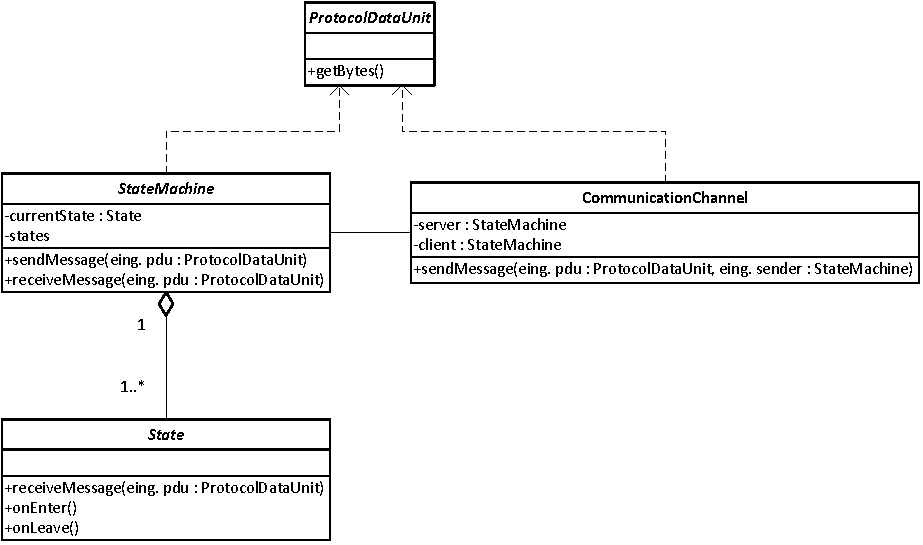
\includegraphics[scale=0.9]{Diagrams/uml/abstract_pdu_state_machine_channel.pdf} %scale=0.8
	\caption{UML-Diagramm der Umsetzung des abstrakten Rahmens}
	\label{fig_uml_abstract_state_machine}
\end{figure}

Für die Übertragung von Nachrichten wird ein \sourceobject{CommunicationChannel}-Objekt genutzt, dass die Übermittlung von Nachrichten zwischen den beiden an dem Protokollablauf beteiligten \sourceobject{StateMachine}-Objekten übernimmt. Außerdem ist in diesem Objekt auch die Thread-Synchronisierung implementiert, die dafür sorgt, dass der Protokollablauf beim Senden einer Nachricht pausiert wird. Dies ermöglicht das schrittweise Verfolgen der gesendeten Nachrichten und der Veränderungen des internen Zustands der Kommunikationspartner. Auch \sourceobject{CommunicationChannel}-Objekte können beobachtet werden, um über zu sendende oder gesendete Nachrichten informiert zu werden.

Um Protokollerweiterungen eine typsichere Umgebung zu bieten, besitzen die \sourceobject{State""Machine}\nobreakdash-, \sourceobject{State}- und \sourceobject{CommunicationChannel}-Klassen einen generischen Parameter vom Typ einer Unterklasse von \sourceobject{ProtocolDataUnit}. Hierdurch können Unterklassen ihren Nachrichtentyp angeben und sich auf die durch Java gewährleistete Typsicherheit verlassen.
\todo{listing of headers?}

% abstract view
\subsubsection{Abstrakte Benutzeroberfläche}
Für die Darstellung des Protokollablaufs wurde ein Gerüst entwickelt, das die im vorherigen Abschnitt beschriebenen Gemeinsamkeiten von Protokollen abbildet. Für die internen Zustände der Parteien wurden zwei Bereiche angelegt, die durch konkrete Protokolle bereitgestellt werden müssen. Außerdem wird eine Liste von bereits gesendeten bzw. als nächstes gesendeten Nachrichten angezeigt, die es  bei Auswahl einer Nachricht ermöglicht, ihre Details anzuzeigen. Dabei wird für jede Nachricht die Darstellung als Bytekette und eine protokollspezifische Detailansicht, die ebenfalls durch konkrete Protokolle bereitgestellt werden muss, angeboten. Zusätzlich kann ein weiteres Fenster angezeigt werden, das es ermöglicht, Informationen zu gewünschten zustands- oder nachrichtenabhängigen Daten darzustellen. Für die Interaktion wurde ein Bedienfeld entwickelt, das die Nachrichtensteuerung bereitstellt und das Informationsfenster öffnet. In der Nachrichtendetaildarstellung können die Bytes einer Nachricht vor dem Senden verändert werden.

Für die Verknüpfung der Datenschicht mit der Benutzeroberfläche wurde das Entwurfsmuster Model-View-Presenter (siehe \cite{potel96}) gewählt, um eine strukturierte Trennung der Schichten zu ermöglichen.

% abstract provider and builder
\subsubsection{Erweiterung der Anwendung}
Um Erweiterungen die Bereitstellung fehlender Elemente und nötiger Objekte zu ermöglichen, wurden die Interfaces \sourceobject{ViewProvider} und \sourceobject{StateMachineProvider} erstellt, die eine Erweiterung implementieren muss. Objekte, die diese Interfaces implementieren, ermöglichen es, das Gerüst mit protokollspezifischen Details zu füllen.\\
\sourceobject{ViewProvider} sorgen für die Bereitstellung von Fensterelementen für die internen Zustände der Parteien, für die Detailansicht einer Nachricht und für optionale Einstellmöglichkeiten zu dem Protokollablauf. \sourceobject{StateMachineProvider} sind zuständig für die entsprechenden \sourceobject{StateMachine}-Objekte für die beiden Parteien. Diese werden dann durch einen \sourceobject{ProtocolBuilder} mit einem \sourceobject{CommunicationChannel} und den entsprechenden Fensterelementen verknüpft. Das UML-Diagramm in Abbildung \ref{fig_uml_abstract_provider_builder} visualisiert diese Zusammenhänge. 

\begin{figure}
	\centering
	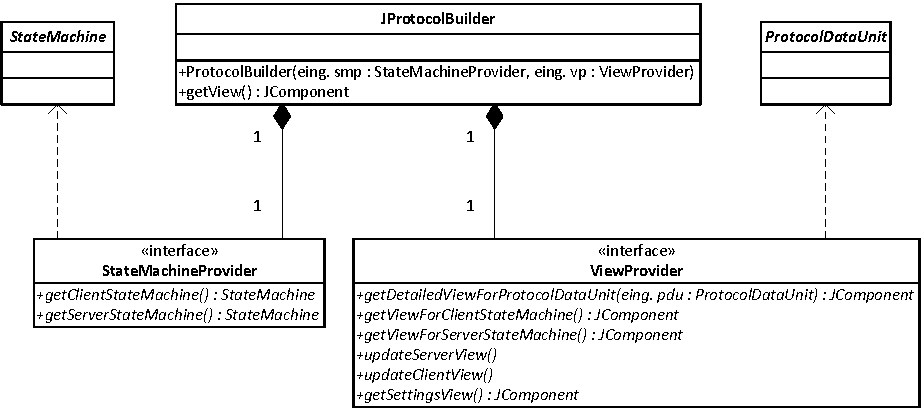
\includegraphics[scale=0.9]{Diagrams/uml/abstract_provider_builder.pdf} %scale=0.8
	\caption{UML-Diagramm von Provider- und ProtocolBuilder-Klassen für die Bereitstellung von Erweiterungen}
	\label{fig_uml_abstract_provider_builder}
\end{figure}

Beim Laden einer neuen Protokollsimulation wird eine Liste vorhandener Protokolle und bei Auswahl eines Eintrags die entsprechende Einstellungsansicht angezeigt. Wenn eine Protokollsimulation gestartet wird, wird das vom \sourceobject{ProtocolBuilder} zur Verfügung gestellte Fensterelement in die Anwendung eingebettet.

\subsection{Erweiterung der Anwendung um TLS 1.2}

% tls 12 model

	% TlsCiphertext and included fragment/message
\subsubsection{Nachrichten}
Als Protokollnachricht dient die Klasse \sourceobject{TlsCiphertext}. Bei ihrer Modellierung wurde versucht, analog zu der Spezifikation vorzugehen und auch Benennungen möglichst einheitlich zu halten. Sie enthält Felder für den \sourceobject{TlsContentType}, die \sourceobject{TlsVersion} und ihre Länge sowie ein \sourceobject{TlsFragment}, das die eigentliche Nachricht der oberen TLS-Protokollschicht enthält.
Abhängig von der aktuellen \ciphersuite{} wird dieses \sourceobject{TlsFragment} verschlüsselt und mit einem MAC versehen. Zusätzlich kann es weitere Felder für bei der Verschlüsselung benötigte Werte enthalten (siehe Abschnitt \ref{sec_record_protocol} und insbesondere Abbildung \ref{fig_tls_cipher_types}). 

Die Nachrichten der oberen Schicht werden durch für jedes Teilprotokoll bestehende Unterklassen von \sourceobject{TlsMessage} dargestellt. Neben \sourceobject{TlsAlertMessage}, \sourceobject{Tls""Change""Cipher""Spec""Message} und \sourceobject{TlsApplicationDataMessage} wurde zusätzlich für jeden HandshakeType eine eigene Klasse erstellt. Alle diese Nachrichten enthalten zwei Konstruktoren, die ihre Erzeugung sowohl aus benötigten Werten als auch durch das Parsen übertragener Bytes ermöglichen. 

	%state machine, states, security paramaters, connection state
\subsubsection{Automatenimplementierung}
Im Folgenden werden die implementierten Klassen für das TLS-Automatenmodell beschrieben. Ein UML-Diagramm dieser Klassen ist in Abbildung \ref{fig_uml_tls_state_machine} zu finden.

Als Unterklasse der \sourceobject{StateMachine}-Klasse wurde \sourceobject{TlsStateMachine} implementiert. Diese Klasse bietet Zugriff auf alle notwendigen, internen Zustandsinformationen von TLS-Client und -Server. Ein Objekt vom Typ \sourceobject{TlsSecurityParameters} bietet Zugriff auf während des Handshakes ausgehandelte Verfahren und Informationen wie SessionId, Random-Werte und das berechnete \mastersecret{}. Objekte vom Type \sourceobject{TlsConnectionState} bilden den current read state und den current write state, sowie den pending state (vgl. Abschnitt \ref{sec_change_cipher_spec}). In ihnen werden ausgehandelte \ciphersuite{} und Schlüssel sowie die aktuelle Sequenznummer verwaltet. Bei Empfang oder nach dem Senden einer \changecipherspec{}-Nachricht kann der pending state zum current state gemacht werden.

Für Client und Server wurden die Unterklassen \sourceobject{TlsClientStateMachine} und \sourceobject{Tls""Server""State""Machine} erstellt, die unterschiedliches Verhalten der beiden Parteien spezifizieren. Insbesondere im Bereich der asymmetrischen Kryptographie sind diese Unterschiede so groß, dass der Mehraufwand gerechtfertigt ist. Beispielsweise besitzt der Server ein RSA-Schlüsselpaar, dessen geheimer Schlüssel zum Entschlüsseln des vom Client ausgewählten \premastersecret{} oder zum Signieren der Diffie-Hellman-Parameter genutzt wird. Der Client ist im Gegensatz dazu lediglich im Besitz des öffentlichen Serverschlüssels zum Verschlüsseln des \premastersecret{}s oder zum Überprüfen der Parametersignatur.

\begin{figure}
	\centering
	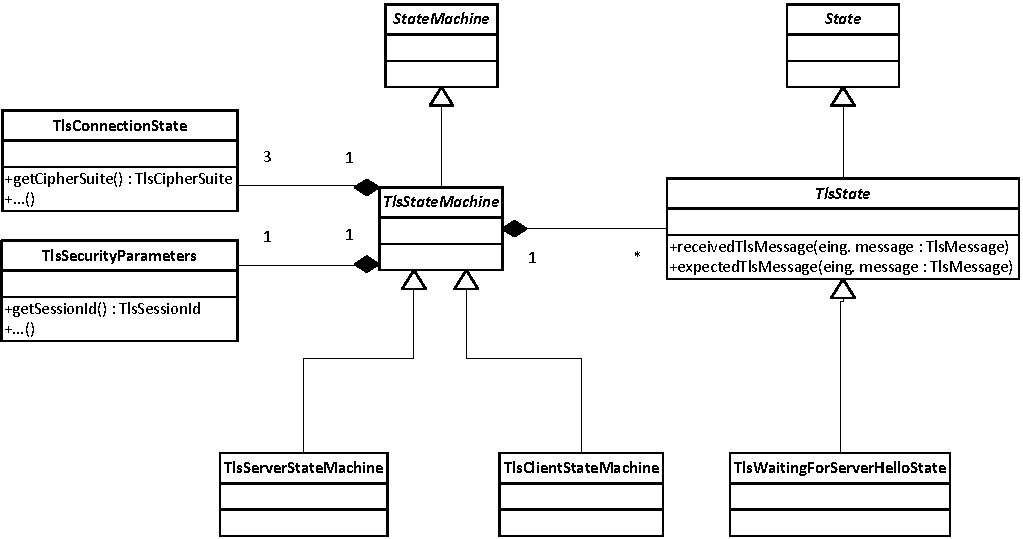
\includegraphics[scale=0.9]{Diagrams/uml/tls_state_machine.pdf} 
	\caption{UML-Diagramm der Klassen für das Tls-Automatenmodell}
	\label{fig_uml_tls_state_machine}
\end{figure}

Entsprechend den Automatenmodellen im Anhang \ref{cha_tls_state_machines} wurden für alle Zustände entsprechende Unterklassen von \sourceobject{TlsState}, einer Unterklasse von \sourceobject{State}, erstellt. Jede dieser Unterklassen definiert die Typen von TLS-Nachrichten der oberen Schicht, die sie erwartet, und implementiert das Verhalten bei Empfang einer solchen Nachricht. Beispielsweise erwartet der Clientzustand \sourceobject{TlsWaitingForServerHelloState} lediglich Handshake-Nachrichten vom Typ \serverhello{}. Bei Empfang einer solchen Nachricht werden die entsprechenden Felder für TlsVersion, ServerRandom, SessionID und \ciphersuite{} gesetzt und der aktuelle Zustand der \sourceobject{TlsClientStateMachine} auf den nachfolgenden Zustand gesetzt. Diese Umsetzung ist in Listing \ref{lst_state_example} zu finden. Nach dem gleichen Prinzip wurde das Verhalten in allen anderen Zuständen implementiert. 

\lstset{style=java, caption={Implementierung des Zustands \sourceobject{TlsWaitingForServerHelloState}}, label=lst_state_example}
\begin{lstlisting}
public class TlsWaitingForServerHelloState extends TlsState {
	...
	%%@Override%%
	public boolean expectedTlsMessage(TlsMessage message) {
		return isHandshakeMessageOfType(message, TlsHandshakeType.server_hello);
	}

	%%@Override%%
	public void receivedTlsMessage(TlsMessage message) {
		...
		setServerHelloValues(message);
		setTlsState(TlsStateType.CLIENT_IS_WAITING_FOR_CERTIFICATE_STATE)
	}

	private void setServerHelloValues(TlsServerHelloMessage message) {
		...
		_stateMachine.setVersion(version);
		_stateMachine.setServerRandom(message.getServerRandom());
		_stateMachine.setSessionId(message.getSessionId());
		_stateMachine.setPendingCipherSuite(message.getCipherSuite());
	}
}
\end{lstlisting}

In der Oberklasse \sourceobject{TlsState} werden eingehende Nachrichten entschlüsselt. Dieser Vorgang wird in dem folgenden Unterabschnitt Kryptographie näher beleuchtet.\\
Danach werden die Nachrichten je nach gesetztem \sourceobject{ContentType} geparst. Fehler bei diesem Vorgang führen zu einem Übergang in einen Fehlerzustand und Senden einer Alert-Nachricht. Anschließend wird überprüft, ob die geparste Nachricht von dem aktuellen Zustand erwartet wird. Ist dies nicht der Fall, so wird ebenfalls ein Fehlerzustand gesetzt und eine Alert-Nachricht gesendet.

	%crypto cipher suites
\subsubsection{Kryptographie}
Im TLS-Protokoll werden die verwendeten Algorithmen und Schlüssellängen durch \ciphersuites{} spezifiziert (siehe Abschnitt \ref{sec_cipher_suites}). Durch das Interface \sourceobject{TlsCipherSuite} werden diese Werte zur Verfügung gestellt. Für die Anwendung wurden verschiedene \sourceobject{TlsCiphersuite}-implementierende Klassen entwickelt, die verschiedene Algorithmen zum Schlüsselaustausch und zur Verschlüsselung beinhalten:
\begin{itemize}
\item TLS\_DHE\_RSA\_WITH\_AES\_128\_CBC\_SHA
\item TLS\_DHE\_RSA\_WITH\_AES\_128\_GCM\_SHA256
\item TLS\_RSA\_WITH\_AES\_128\_CBC\_SHA
\item TLS\_RSA\_WITH\_AES\_128\_GCM\_SHA256
\end{itemize}
Durch diese Wahl der \ciphersuites{} können sowohl der Diffie-Hellman- als auch der RSA-Schlüsselaustausch beobachtet werden. Außerdem ist die Verschlüsselung per Blockchiffre (AES im CBC-Modus) oder AEAD-Chiffre (AES im GCM-Modus) möglich.

Für die kryptographischen Algorithmen wurde auf die Implementierungen der Java-Bibliothek zurückgegriffen. Die TLS-spezifische PseudoRandomFunction wurde eigenständig entwickelt und durch Testvektoren auf ihre Richtigkeit hin überprüft.\\
Ebenso wurde auch die Verknüpfung der Algorithmen für die Ver- und Entschlüsselung, also beispielsweise die Berechnung von MAC, Padding und Paddinglänge und die anschließende Verschlüsselung, für Block- und AEAD-Chiffren selber in den Klassen \sourceobject{TlsBlockCipherSuite} und \sourceobject{TlsAeadCipherSuite} implementiert. Konkrete \ciphersuites{} füllen lediglich die vorgegebenen Rahmen und bieten Zugriff auf Schlüssellängen und die verwendeten Algorithmen.

In der \sourceobject{TlsState}-Klasse werden zu sendende Nachrichten durch die im current write state gesetzte \ciphersuite{} von \sourceobject{TlsPlaintext}- in \sourceobject{TlsCiphertext}-Objekte umgewandelt und anschließend gesendet. Beim Empfang von Nachrichten wird dieser Prozess umgekehrt durchlaufen. Bei auftretenden Fehlern wie einem falschen Schlüssel oder einem ungültigen MAC erfolgen wiederum der Übergang in einen Fehlerzustand und das Senden einer Alert-Nachricht.

% tls 12 view
\subsubsection{Benutzeroberfläche}
\begin{figure}
	\centering
	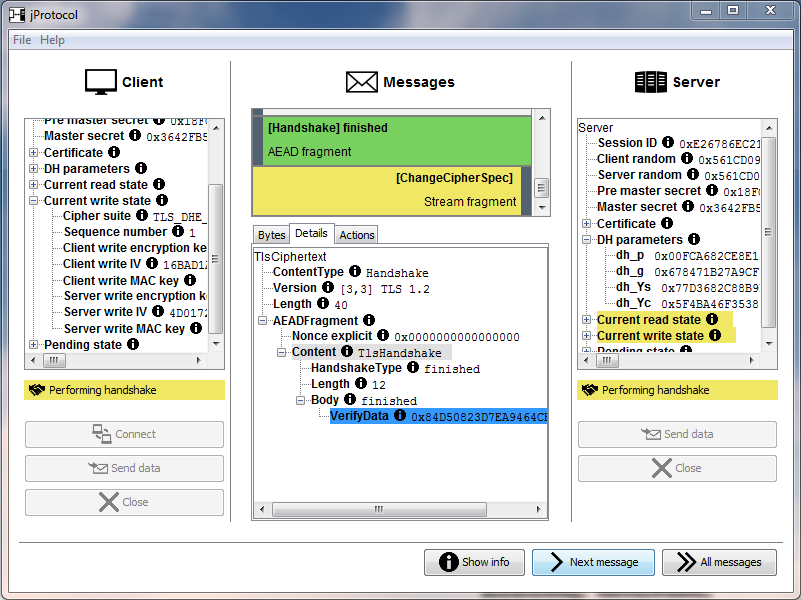
\includegraphics[scale=0.7]{Diagrams/ScreenshotTLS.png} 
	\caption{Die fertige Anwendung}
	\label{fig_application_screenshot}
\end{figure}

Den Überlegungen im vorherigen Abschnitt entsprechend wurde für die Benutzeroberfläche von Client und Server ein auf der Swing-Komponente \sourceobject{JTree} basierendes Fensterelement entwickelt. Der interne Zustand der Parteien wird durch Titel-Wert-Paare und optionale Kindelemente dargestellt. Die Klasse \sourceobject{TlsStateMachine} enthält eine Methode, die die Paare für den aktuellen Zustand zurückliefert.\\
Bei Zustandsänderungen, die durch das Beobachter-Muster kommuniziert werden, werden der alte und neue Zustand verglichen und neue oder geänderte Einträge gekennzeichnet, sodass Auswirkungen von empfangenen Nachrichten sichtbar werden.\\
Zusätzlich wurde zu den jeweiligen Einträgen jeweils ein erklärender Informationstext mit Auszügen aus der Spezifikation erstellt, um ein besseres Verständnis der Abläufe zu unterstützen.\\
Zusätzlich enthalten die Fensterelemente Buttons für die verfügbaren Aktionen wie das Verbinden oder das Senden von Daten bei bestehender Verbindung.

Das gleiche Fensterelement wie für Server und Client wurde auch für die Detaildarstellung von Nachrichten verwendet. Auch für die jeweiligen Nachrichtenfelder sind Informationstexte erstellt worden, die beim Verstehen der Protokolls helfen sollen.

Ein Screenshot der endgültigen Anwendung mit der Erweiterung um TLS ist in Abbildung \ref{fig_application_screenshot} zu finden.